\documentclass[11pt,a4paper]{article}
\usepackage[T1]{fontenc}
\usepackage{lmodern}
\usepackage[latin1]{inputenc}
\usepackage{a4wide}
\usepackage[dvips]{graphicx}
\usepackage{float}

\usepackage[
pdfauthor={ace project team},
pdftitle={Network Analysis Report},
pdfcreator={pdftex},
]{hyperref}

\usepackage{sectsty}
\allsectionsfont{\sffamily}

\usepackage{fancyheadings} 
\pagestyle{fancy} 
\lhead{\textsf{\textbf{ACE} \\ \small{a collaborative editor}}}
\chead{}
\rhead{
\includegraphics[height=0.875cm,width=3cm]{../../images/logo_BFH.eps}}
\lfoot{}
\cfoot{\textsf{\thepage}}
\rfoot{}
\setlength{\headrulewidth}{0.6pt}
\setlength{\footrulewidth}{0.6pt}
\setlength{\topmargin}{-50pt}
\addtolength{\headheight}{50pt}

\usepackage{colortbl}

\newcommand{\headercol}[2]{\multicolumn{1}{|>{\bfseries\columncolor[gray]{0.82}}p{#1}|}{\textsf{#2}}}
\newcommand{\ace}[0]{\emph{ACE }}



\begin{document}
\setlength{\parindent}{0pt}

\begin{titlepage}
\thispagestyle{empty}
  \includegraphics[height=1.5in]{../../images/pix.eps}

  \begin{center}

    {\fontsize{40}{45} \textbf{\textsf{ACE}}} \\
    \textsf{a collaborative editor} \\
        
    \vspace{36pt}
        
    {\huge{\textbf{\textsf{Report Evaluation Network}}}} \\

    \vspace{36pt}

	\textsf{Berne University of Applied Sciences} \\
    \textsf{School of Engineering and Information Technology} \\
    
  \end{center}

  \vfill
  
  \begin{tabular}{ll}
   \hline

   \\

   \multicolumn{1}{>{\bfseries}p{1.5in}}{\textsf{Date:}} &
   \multicolumn{1}{>{}p{4.3in}}{\textsf{14.06.2005}}          \\
   
   \\
   
   \multicolumn{1}{>{\bfseries}p{1.5in}}{\textsf{Version:}}     &   
   \multicolumn{1}{>{}p{4.3in}}{\textsf{0.6}}                 \\

   \\
   
   \multicolumn{1}{>{\bfseries}p{1.5in}}{\textsf{Projectteam:}}                 &
   \multicolumn{1}{>{}p{4.3in}}{\textsf{Mark Bigler (biglm2@hta-bi.bfh.ch)}}  \\
   \multicolumn{1}{>{\bfseries}p{1.5in}}{}                                      &
   \multicolumn{1}{>{}p{4.3in}}{\textsf{Simon R�ss (rasss@hta-bi.bfh.ch)}}    \\
   \multicolumn{1}{>{\bfseries}p{1.5in}}{}                                      &
   \multicolumn{1}{>{}p{4.3in}}{\textsf{Lukas Zbinden (zbinl@hta-bi.bfh.ch)}} \\   
   
   \\
   
   \multicolumn{1}{>{\bfseries}p{1.5in}}{\textsf{Receivers:}}                       &
   \multicolumn{1}{>{}p{4.3in}}{\textsf{Jean-Paul Dubois (doj@hta-bi.bfh.ch)}}       \\
   \multicolumn{1}{>{\bfseries}p{1.5in}}{}                                          &
   \multicolumn{1}{>{}p{4.3in}}{\textsf{Claude Fuhrer (frc@hta-bi.bfh.ch)}}       \\

   \\
   
   \multicolumn{1}{>{\bfseries}p{1.5in}}{\textsf{Location:}}               &   
   \multicolumn{1}{>{}p{4.3in}}{\textsf{Subversion Repository}} \\

   \\  
   
   \hline
  \end{tabular}

\end{titlepage}

\newpage

\tableofcontents
\newpage

\listoftables
\listoffigures
\newpage


\section{Introduction}
The goal of the semester project is to create a fully functional operational transformation algorithm. We are implementing the \emph{Jupiter} algorithm. In the diploma project we will (most likely) build a collaborative text editor that uses this algorithm. One of the most central things to implement will be a network layer. The requirements for this layer will be detailed later (see \ref{sect:requirements}). But first let's define the purpose of this document.

\subsection{Purpose}
The purpose of this document is to examine existing networking solutions and to gather information so that we can decide how to implement the network layer of \ace. It is not a goal to select a network technology for \ace yet. This decision can be delayed further. 

\subsection{Requirements}
\label{sect:requirements}
The network layer will need to provide the following two basic features:

\begin{itemize}
 \item discovery
 \item communication
\end{itemize}

Let us explain these two basic points in greater detail.

\subsubsection{Discovery}
In \ace a user will be able to share a document so others can join him editing this document. Without a way of first advertising a shared document and then discovering it, the application is pretty useless. The discovery should be as simple as possible. There are several technologies that allow automatic discovery of services, for instance \emph{Jini}, \emph{Bonjour} (also known as zero-conf networking) and diverse peer-to-peer frameworks (e.g. \emph{JXTA}).

\subsubsection{Communication}
This is the basic requirement. When a user discovered a shared document and decided to join that document, there must be a way to communicate between the document publisher and the user that wants to join the document. There are different technologies ranging from plain socket communication over remote method invocation to complex peer-to-peer frameworks. They differ in several aspects such as ease of use and platfrom independence.

The \emph{Jupiter} algorithm does not need a network layer that is capable of multicast. Each operation is sent to the server only. Clients must not be explicitely aware of other users editing the same document from the viewpoint of the algorithm. That is why some network technologies targeting multicast communication are most likely not an appropriate choice (although they would be for an algorithm that requires multicast messaging).



\section{General Aspects}
Ideally, every user could publish a document that could be discovered by other users no matter where they are. However, the Internet poses some issues that make this ideal world hard to accomplish. In the following sections we will first analyze the fundamental problems we face when deploying a distributed application on the Internet and then propose some ways how one could deal with them.

\subsection{Firewalls/NAT}
Most Internet users today do not have public IP addresses. They are behind a NAT (network address translation) router and sometimes behind firewalls too (e.g. corporate users). If a user wants to publish a document, there must be some kind of server that accepts connections for the given document. If the server is behind a NAT router, there is usually way an external client can connect to that document server. If the server is behind a firewall, the situation is even more problematic as the firewall will most likely block most incoming traffic. The basic dilemna with NAT routers and firewalls is depicted in figure \ref{fig:firewall}.

\begin{figure}[H]
 \centering
 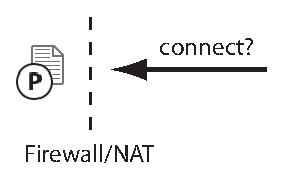
\includegraphics[width=4.2cm,height=2.6cm]{../../images/net_firewall.eps}
 \caption{Basic Problem with Firewalls and NAT Routers}
 \label{fig:firewall}
\end{figure}

\subsection{Tunneling Firewalls}
It would be possible to tunnel firewalls, although this technique is a bit delicate. Firewalls are there for a reason. Tunneling firewalls is most likely against the will of the security policy of a company. So this is not considered to be a requirement for our application.

\subsection{Dealing with NAT Router}
The problem with NAT routers is, that nobody from the outside can connect to a computer on the inside. Of course it would be possible to set up the router in a way that it delegates requests for certain services to one particular computer, but we do not consider this as an acceptable technique for an end user application. We cannot expect endusers to do this setup.

The solution to this problem is, that the client must establish the connection first to a host outside of the local network. If we consider the basic use case where a user wants to publish a document so others can join him editing it. There are some possibilities.

\subsubsection{Proxy Host}
Let us say there is a host P, called proxy in the following, and a host A, called the publisher. Host A sits behind a NAT router and wants to publish a document. In this solution host A connects to the proxy host P which publishes the document in stead of A. Every other client that wants to join the document published by A connects to P instead. P acts as a proxy and forwards all requests to A. P also forwards any responses from A to all the other clients of this editing session.

This solution to the NAT problem is depicted by figure \ref{fig:proxy}.

\begin{figure}[H]
 \centering
 
\includegraphics[width=3.8cm,height=2.9cm]{../../images/net_proxy.eps}
 \caption{Solution to NAT Problem: Proxy Host}
 \label{fig:proxy}
\end{figure}

\subsubsection{Substitute Host}
Let us say there is a host S, called substitute in the following, and a host A, called the publisher. Host again sits behind a NAT router and wants to publish a document. In this solution host A connects to the proxy host S which publishes the document and hosts the document itself. So the host A is no longer the publisher of the document, but merely an ordinary client. Host S plays the substitute of host A because he has a public IP address whereas host A has not.

The substitute host solution to the NAT problem is depicted by figure \ref{fig:substitute}. It is very similar to the proxy host solution. The only difference is, that the substitute host is itself the server whereas the proxy host is only a proxy forwarding all requests back to the publisher host A.

\begin{figure}[H]
 \centering
 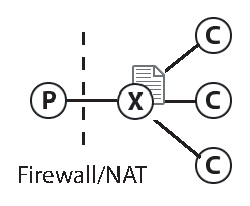
\includegraphics[width=3.7cm,height=2.9cm]{../../images/net_substitute.eps}
 \caption{Solution to NAT Problem: Subsitute Host}
 \label{fig:substitute}
\end{figure}


\subsection{Document Publishing}
When a user publishes a document, he wants other users to find it. There must be some kind of discovery mechanism that allows users to discover published documents. There are several solutions for this problem. On the LAN clients could use IP multicast to discover documents (see section \ref{sect:jini} and section \ref{sect:bonjour}). IP multicast usually fails in WANs because routers block multicast traffic. A common and relatively straightforward solution for WANs would be to have a (or several load-balancing) central servers that manage all the document advertisements. A pure P2P solution could build upon a P2P framework (see section \ref{sect:jxta}) to avoid central servers at all.




\section{JGroups}
\emph{JGroups} is a toolkit for reliable multicast communication. It can be used to create groups of processes whose members can send messages to each other. The main features include:

\begin{itemize}
 \item Group creation and deletion (members can spread across LANs or WANs).
 \item Joining and leaving groups.
 \item Membership detection and notification about joined/left/crashed members
 \item Detection and removal of crashed members
 \item Sending and receiving of member-to-group messages (point-to-multipoint)
 \item Sending and receiving of member-to-member messages (point-to-point)
\end{itemize}

One of the most powerful features of \emph{JGroups} is its flexible protocol stack, which allows developers to adapt it to exactly match the application requirements and network characteristics. The benefit of this is that one has only to pay for what is actually used. By mixing and matching protocols, various differing application requirements can be satisfied. \emph{JGroups} comes with a number of protocols, for example

\begin{itemize}
 \item Transport protocols: UDP (IP multicast), TCP, JMS
 \item Fragmentation of large messages
 \item Reliable unicast and multicast message transmission. Lost messages are
       retransmitted.
 \item Failure detection: crashed members are excluded from membership
 \item Ordering protocols: atomic (all-or-none message delivery), FIFO, causal,
       total order (sequencer or token based)
 \item Membership
 \item Encryption
\end{itemize}

\emph{JGroups} allows developers to create reliable multicast applications where
\emph{reliability} is a deployment issue and does not have to be implemented by the application developer. This saves application developers significant amounts of time and allows for the application to be deployed in different environments without having to change code.

\subsection{Basics}
In order to join a group and send messages, a process has to create a channel. A channel is similar to a socket. When a client connects to a channel, it gives the name of the group it would like to join. A channel is always associated with a particular group (in it's connected state). The protocol stack takes care that channels within the same group find each other. Whenever a client connects to a channel with group name G, then it tries to find existing channels with the same name and joins them. If no members exist, a new group will be created.

When a channel is created, it is first in the unconnected state. The clients connects to the channel by calling \texttt{connect} supplying the group name that it wants to join. Once the channel is in the connected state, messages can be sent/received. A channel can be disconnected from a group by calling \texttt{disconnect} and it can be closed by calling \texttt{close}. A closed channel cannot be used anymore. Any attempt to do so results in an exception. The channel can only be connected to one group at the time. To communicate with multiple groups, multiple channels have to be created.

\subsubsection{Creating a channel}
To create a channel we can use the public constructor of \texttt{JChannel}. It looks as follows:

\begin{verbatim}
public JChannel(Object properties) throws ChannelException
\end{verbatim}

The properties arguments defines the composition of the protocol stack, that is the number and types of layers, their parameters and their order. For \texttt{JChannel} this has to be a string. For details about the composition of this string, please refer to the \emph{JGroups} users guide.

\subsubsection{Sending messages}
One of the two \texttt{send} methods of a channel are used to send messages to group members. The message payload can be any serializable object.

\begin{verbatim}
JChannel channel = ...;
channel.send(null, null, "test");
\end{verbatim}

The above code fragment sends the string "test" to all the other members in the group.

\subsubsection{Receiving messages}
The \texttt{receive} method is used to receive messages. A channel receives messages asynchronously from the network and stores them in a queue. When receive is called, the first message in the queue is removed and returned. If there is no message in the queue, the method invocation blocks.

There is a so-called \emph{building block} that provides a listener interface for receiving messages. The building block is called \texttt{PullPushAdapter}. This relieves the application developer from the task to create a separate reception thread. 

\subsection{Analysis}
\emph{JGroups} provides a very simple API to create groupware applications. A shared document in \ace could be represented as a separate group in \emph{JGroups}. 

\subsubsection{Shortcomings}
To join a group, one has to know the name of the group to join. There would have to be some mechanism to discover the available groups, or more specifically, the available groups that represent shared documents in \ace. A central server could be used to register group names or a well-known group could be used to advertise/query for available documents.

The current implementation of the group membership service is very simplistic. Joining a group is always successul. There is no way to forbid a particular member the access the group. This is a serious problem as the confidentiality of the document content cannot be guaranteed. A custom group membership service protocol implementation could probably solve this particular problem.

The \emph{JGroups} library is not programming language independent. It uses serialized objects as message payload. This can be seen as and advantage or as a disadvantage depending on the requirements of the application.

\section{Rendezvous / Bonjour}
\emph{Bonjour}, formerly known as \emph{Rendezvous}, enables automatic discovery of computers, devices, and services on IP networks. It uses industry standard IP protocols to allow devices to automatically discover each other without the need to enter IP addresses or configure DNS servers. It is a technology developed by Apple that is submitted to the IETF as part of an ongoing standards-creation process. The technology is more generally known as zero-conf networking.

There are \emph{Java} libraries available that allow to use this technology in any \emph{Java} application. The library needs a native library that is available for all major platforms. 

DNS service discovery is a way of using standard DNS programming interfaces, servers, and packet formats to browse the network for services. It is compatible with, but not dependent on, multicast DNS. Multicast DNS is a way of using familiar DNS programming interfaces, packet formats and operating semantics, in a small network where no conventional DNS server has been installed.

\subsection{Prototype}
The technology is best described by a simple prototype. We've created a simple echo server and echo client that show off the basic features of this technology.

\subsubsection{Echo Server}
The echo server is implemented in the class \texttt{ch.iserver.ace.net.bonjour.EchoServer}. It is very similar to normal echo server implementation. First a \texttt{ServerSocket} is created listening on a particular socket. Then the service is registered with DNS service discovery system represented by the \texttt{com.apple.dnssd.DNSSD} class. A listener (\texttt{com.apple.dnssd.RegisterListener}) is used to inform the application when the registration was successull. Once the registration was successul, the echo server starts to service clients as any echo server would do.

\subsubsection{Echo Client}
The echo client (see \texttt{ch.iserver.ace.net.bonjour.EchoClient}) is a simple GUI that allows to send echo requests to echo servers. It browses the network for available echo servers and lists them in a combo box. The user can select one of those echo servers and send an echo request to them.

The method \texttt{browse} of the \texttt{DNSSD} class is used to issue a browse request to the DNS service discovery system. We have to supply a \texttt{com.apple.dnssd.BrowseListener} implementation that gets called back whenever a service of specified type is found.

Whenever the user sends a message to the currently selected echo server by entering a message in the bottom textfield and hitting enter, the service has to be resolved. This happens by calling \texttt{resolve} on the \texttt{DNSSD} class. The application is called back over a \texttt{com.apple.dnssd.ResolveListener}. The method \texttt{serviceResolved} is called on this listener when the service is resolved. This provides us with the service name, host name and port of the service. As a last step we have to get the IP address of the service. This is done by calling \texttt{queryRecord} on the \texttt{DNSSD} class. We get called back by a method call to \texttt{queryAnswered} in the \texttt{com.apple.dnssd.QueryListener} we supplied to the \texttt{queryRecord} call.

At that point we do have enough information to contact the echo server and send the echo request over a plain socket connection. That's one important point to observer. This technology enables us to discover services on the network but does not impose any limitations on the way we communicate from client to server.
\section{Jini/RMI}
In a running \emph{Jini} system, there are three main players. There is a service, a client which would like to make use of services and a lookup service (service locator) which acts as a broker/locator between services and clients. Clients can query lookup services to dynamically discover services. Services register themselves with a lookup service so that they can be discovered by clients. The communication from client to service happens usually through a service proxy that communicates with RMI to the real service (although it could use any protocol).



\subsection{Analysis}
\emph{Jini/RMI} fulfills all our requirements, discovery and communication. Services are discovered through the lookup service. The lookup service is discovered either through unicast connections (in case that the lookup service is known in advance) or through multicast messages. A shared document could be represented as a document service that is registered in the lookup service.

\subsubsection{Positive Points}
We studied \emph{Jini} and \emph{RMI} in a semester course. So these technologies are known well enough to implement the network layer with them.

A network layer based on \emph{Jini/RMI} would be relatively straightforward. The whole system would be based on Java.

\subsubsectoin{Negative Points}
\emph{Jini} relies on a JVM at each site, although not the whole system has to be implemented in \emph{Java} (e.g. services can be implemented in other programming languages). This is a serious drawback if we want to make \ace interoperable.

\subsubsection{Open Points}
There are no open points (besides designing the software).

\subsubsection{Jini vs. Bonjour}
At that point, it would be interesting to compare \emph{Jini} with \emph{Bonjour} (aka zero-conf networking). Both provide ways to dynamically discover services. One obvious difference is that \emph{Bonjour} does not rely on a JVM. Programs written in most programming language can discover services with it, as it is an extension to the domain name system (DNS). This is also one of the most obvious limitations of \emph{Bonjour} technology. \emph{Bonjour} can only discover that what could be stored in a traditional \emph{DNS} server. Usually all that is discovered through \emph{Bonjour} is an IP address and port number. It is then up to the client to know what to do with this information. If it does not know the protocol used to connect to that particular service, the information is pretty useless.

\emph{Jini} on the other hand downloads a service object (usually a proxy object). The service object itself either does the requested work itself or in case of a proxy knows how to communicate with the real service. All the client has to know is the service interface (a Java interface).

It is this transfer of service object that makes \emph{Jini} so much more powerful than \emph{Bonjour} technologies. Interesting enough, \emph{Bonjour} seems to be much more widely used than \emph{Jini}, most likely because it does not depend on a JVM.



\subsection{Resources}
\begin{itemize}
 \item \url{http://www.jini.org/}
\end{itemize}

\section{JXTA}
\label{sect:jxta}

\emph{JXTA} technology is a set of open protocols that allow any connected device on the network ranging from cell phones and wirless PDAs to PCs and servers to communicate and collaborate in a P2P manner.

\emph{JXTA} peers create a virtual network where any peer can interact with other peers and resources directly even when some of the peers and resources are behind firewalls and NATs or are on different network transports.

The project objectives of \emph{JXTA} are:
\begin{itemize}
 \item Interoperability - across different peer-to-peer systems and communities
 \item Platform independence - multiple/diverse languages, systems and networks
 \item Ubiquity - every device with a digital heartbeat
\end{itemize}


\subsection{Concepts}

\subsubsection{Peers}
A \emph{peer} is any networked device that implements one or more of the \emph{JXTA} protocols. Peers can include phones, PDAs, as well as PCs, servers and supercomputers. Each peer operates independently and asynchronously from all other peers, and is uniquely identified by a peer ID.

Peers are not required to have direct point-to-point network connections between themselves. Intermediary peers may be used to route messages to peers that are separated due to physical network connections or network configuration (e.g. NATs, firewalls, proxies).

Peers are typically configured to spontaneously discover each other on the network to form transient or persistent relationships called peer groups.

\subsubsection{Peer Groups}
A \emph{peer group} is a collection of peers that have agreed upon a common set of services. Peers self-organize into peer groups, each identified by a unique peer group ID. Each peer group can establish its own membership policy from open (anybody can join) to highly secure and protected (sufficient credentials are required to join).

Peers may belong to more than one peer group simultaneously. By default, the first group that is instantiated is the Net Peer Group. All peers belong to the Net Peer Group. Peers may elect to join additional peer groups.

There are several motivations fro creating peer groups:
\begin{itemize}
 \item \emph{To create a secure environment}: Groups create a local domain of control in which a specific security policy can be enforced. The security policy may be as simple as a plain text user name/password exchange, or as sophisticated as public key cryptography. Peer gropus form logical regions whose boundaries limit access to the peer group resources.
 \item \emph{To create a coping environment}: Groups allow the establishment of a local domain of specialization. For example, peers may group together to implement a document sharing network or a CPU sharing network.
 \item \emph{To create a monitoring environment}: Peer groups permit peers to monitor a set of peers for any special purpose (e.g. traffic introspection, accountability) 
\end{itemize}

A peer group provides a set of services called peer group services. \emph{JXTA} defines a core set of peer group services. Additional services can be developed for delivering specific services. In order for two peers to interact via a service, they must both be part of the same peer group.

\subsubsection{Core Peer Group Services}
The core peer group services include the following:
\begin{itemize}
 \item \emph{Discovery Service} - The discovery service is used by peer members to search for peer group resources, such as peers, peer groups, pipes and services.
 \item \emph{Membership Service} - The membership service is used by current members to reject or accept a new group membership application. Peer wishing to join a peer group must first locate a current member, and then request to join. The application to join is either rejected or accepted by the collective set of current members. The membership service may enforce a vote of peers or elect a designated group representative to accept or reject new membership applications.
 \item \emph{Access Service} - The access service is used to validate requests made by one peer to another. The peer receiving the request provides the requesting peers credentials and information about the request being made to determine if the access is permitted.
 \item \emph{Pipe Service} - The pipe service is used to create and manage pipe connections between the peer group members.
 \item \emph{Resolver Service} - The resolver service is used to send generic requests to other peers. Peers can define and exchange queries to find any information that may be needed (e.g. the status of a service).
 \item \emph{Monitoring Service} - The monitoring service is used to allow one peer to monitor other members of the same peer group.
\end{itemize}

Not all the above services must be implemented by every peer group. A peer group is free to implement only the services it finds useful, and rely on the default net peer group to provide generic implementations of non-critical core services.

\subsubsection{Network Services}
Peers cooperate and communicate to publish, discover, and invoke network services. Peers can publish multiple services. Peers discover network services via the Peer Discovery Protocol. 

The JXTA protocols recognize two levels of network services:
\begin{itemize}
 \item \emph{Peer Services}: A peer service is accessible only on the peer that is publishing that service. If that peer should fail, the service also fails. Multiple instances of the service can be run on different peers, but each instance publishes its own advertisement. 
 \item \emph{Peer Group Services}: A peer group service is composed of a collection of instances (potentially cooperating with each other) of the service running on multiple members of the peer group. If any one peer fails, the collective peer group service is not affected (assuming the service is still available from another peer member). Peer group services are published as part of the peer group advertisement. 
\end{itemize}

\subsubsection{Pipes}
JXTA peers use pipes to send messages to one another. Pipes are an asynchronous and unidirectional non reliable (with the exception of unicast secure pipes) message transfer mechanism used for communication, and data transfer. Pipes are indiscriminate; they support the transfer of any object, including binary code, data strings, and Java technology-based objects. 

The pipe endpoints are referred to as the input pipe (the receiving end) and the output pipe (the sending end). Pipe endpoints are dynamically bound to peer endpoints at runtime. Peer endpoints correspond to available peer network interfaces (e.g., a TCP port and associated IP address) that can be used to send and receive message. JXTA pipes can have endpoints that are connected to different peers at different times, or may not be connected at all. 

Pipes are virtual communication channels and may connect peers that do not have a direct physical link. In this 
case, one or more intermediary peer endpoints are used to relay messages between the two pipe endpoints. 
Pipes offer two modes of communication, point-to-point and propagate, as seen in . The JXTA core also provides 
secure unicast pipes, a secure variant of the point-to-point pipe. 

\begin{itemize}
 \item \emph{Point-to-point Pipes}: A point-to-point pipe connects exactly two pipe endpoints together: an input pipe on one peer receives messages sent from the output pipe of another peer, it is also possible for multiple peers to bind to a single input pipe. 
 \item \emph{Propagate Pipes}: A propagate pipe connects one output pipe to multiple input pipes. Messages flow from the output pipe (the propagation source) into the input pipes. All propagation is done within the scope of a peer group. That is, the output pipe and all input pipes must belong to the same peer group. 
 \item \emph{Secure Unicast Pipes}: A secure unicast pipe is a type of point-to-point pipe that provides a secure, and reliable communication channel. 
\end{itemize}

\subsubsection{Bidirectional reliable communication channels}
Since pipes provide unidirectional, unreliable communication channels, it is necessary to implement bidirectional and reliable communication channels. The platform provides the following to address the level of service quality required by the applications
\paragraph{Reliability Library:} Ensures message sequencing, delivery and exposes message and stream based interfaces.
\paragraph{JxtaSocket and JxtaServerSocket:} Provides \texttt{Socket} and \texttt{ServerSocket} implementations built on top of pipes and the reliability library. It exposes the well knwon stream based interface for communication. Furthermore it provides bidirectional and reliable communication channels.
\paragraph{JxtaBiDiPipe and JxtaServerPipe:} Is built ont top of pipes and the reliability library. It provides bidirectional and reliable communication channels and exposes a message based interface.

\subsubsection{Messages}
A message is an object sent between \emph{JXTA} peers. It is the basic unit of data exchange between peers. Messages are sent and received by the Pipe Service and by the Endpoint Service. Typically, applications use the Pipe Service to create, send and receive messages. 

A message is an ordered sequence of named and typed contents called message elements. Thus a message is essentially a set of name/value pairs. The content can be an arbitrary type. 

The JXTA protocols are specified as a set of messages exchanged between peers. Each software platform binding describes how a message is converted to and from a native data structure such as a Java technology object or a C structure. 

\subsubsection{Advertisements}
All \emph{JXTA} network resources - such as peers, peer groups, pipes and services - are represented by an \emph{advertisement}. Advertisements are language-neutral meta-data structures represented as XML documents. The \emph{JXTA} protocols use advertisements to describe and publish the existence of peer resources. Peers discover resources by searching for their corresponding advertisements, and may cache any discovered advertisements locally.

Each advertisement is published with a lifetime that specifies the availability of its associated resource. Lifetimes enable the deletion of obsolete resources without requiring any centralized control. An advertisement can be republished (before the original advertisement expires) to extend the lifetime of a resource.

\subsubsection{Security}
Dynamic P2P networks such as the \emph{JXTA} network need to support different levels of resource access. \emph{JXTA} peers operate in a role-based trust model, in which an individual peer acts under the authority granted to it by another trusted peer to perform a particular task. 

\subsubsection{IDs}
Peers, peer groups, pipes and other \emph{JXTA} resources need to be uniquely identifiable. A \emph{JXTA} ID uniquely identifies an entity and serves as a canonical way of referring to that entity. 



\subsection{Prototype}
The prototype is a very simple sample application from the programmers guide. There are two classes, \texttt{ch.iserver.ace.net.jxta.Server} and \texttt{ch.iserver.ace.net.jxta.Client}. The server first advertises a service, which the client discovers and sends a simple message to it. The communication is strictly unidirectional (and unreliable, as it is using pipes). The example could certainly be extended to provide a bidirectional and reliable service (e.g. to create an echo server, client).

The server creates first a new module class advertisement and publishes it both locally and remotely (using the discovery service). Afterwards it creates a module specification advertisement. A pipe advertisement is read from the filesystem and attached to the module specification advertisement. This module specification advertisement is then also published locally and remotely.

The server then creates an input pipe from the pipe advertisement and waits for messages on this pipe in an endless loop.

The client first tries to discover the module specification advertisement published by the server. It queries for this advertisement by specifying a value (JXTASPEC:JXTA-EX1) for the name attribute of the specification. The advertisement can be already cached locally. In this case, the client does not need to send a discovery request. If the advertisement is not cached, it sends a discovery request to the network.

Once the client has retrieved the desired module specification advertisement, it can extract the pipe advertisement from the specification advertisement. The pipe advertisement is then used to create an output pipe. The output pipe provides a way of sending a message to the server. When the message is sent successfully, the client shuts down.



\subsection{Analysis}
\emph{JXTA} does certainly sound very promising. It provides some features that seem very interesting for our application. 

\emph{JXTA} satisfies both requirements, discovery and communication. It could be used on its own to create the whole network layer for \ace.

\subsubsection{Positive Points}
One of the most interesting features of \emph{JXTA} is its capability to penetrate firewalls and pass through NAT routers. This means that a user can share a document even if he is behind a NAT router and/or a firewall. The advertisement of a shared document can still be found from the outside. No central server is required to achieve this. \emph{JXTA} employs so called router and rendezvous peers, some special type of peers, to achieve this characteristic.

By avoiding the use of a central server, there is no single point of failure. If our editor's network implementation would be based on \emph{JXTA}, no additional setup would be required for users (setup of server). A user could download an application and would be capable of directly using it.

Further \emph{JXTA} is programming language independent. There is an implementation of the \emph{JXTA} protocols for \emph{Java} as well as there is one for \emph{C}. XML is used a lot in protocol messages, although this is not strictly necessary for custom services.

\subsubsection{Negative Points}
Although \emph{JXTA} exists since 2001 there do not seem to be many applications using it. Only a handful applications are listed on the jxta.org homepage.

Another discomforting point is that we've stumbled across a serious bug in a so called stable release (2.3.3). A clone method caused a stack overflow exception and we had to use the latest build. The bug is even observable in an official sample application presented in the programmers guide.

It seems to us that \emph{JXTA} is still in some way a research project and not rock solid and mature.

\subsubsection{Open Points}
Before we could decide to use \emph{JXTA} for the implementation of the network layer, we would need to explore this technology in greater detail:

\paragraph{Performance:} We don't have much experience with this technology. Although the capabilities seem great, the question remains whether the overhead introduced by them is acceptable. Two separate aspects would have to be tested: (i) discovery performance and (ii) communication performance. The first point concerns itself with the question, how long it would take to find a published advertisement (e.g. a shared document). The second point concerns the communication throughput and latency once a connection (i.e. a pipe) has been connected.

\paragraph{Application:} How would we map the desired network functionality of \ace (publish document, join document, leave document) to \emph{JXTA}?

\paragraph{Membership Service:} The \emph{JXTA} documents mention that a custom implementation of the membership service can be used to decide who is allowed to join a group (a document) and who is not. Different possibilities exist, e.g. voting in a group or decision of the document owner.

\paragraph{Security:} \emph{JXTA} seems to provide security services (e.g. transport layer security). It would certainly be interesting to make all communication within a group confidential.



\subsection{Resources}
\begin{itemize}
 \item \url{http://www.jxta.org/} - \emph{JXTA} project website
 \item \url{http://www.brendonwilson.com/projects/jxta/} - free book, slighlty outdated
 \item \url{http://www.javaworld.com/javaworld/jw-05-2005/jw-0509-jxta.html} - Java World article
 \item \url{http://www.developer.com/java/other/article.php/1450221} - article from developer.com
\end{itemize}

\section{BEEP}
\emph{BEEP} stands for Blocks Extensible Exchange Protocol. It is a protocol framework for building application protocols. Many Internet protocols reinvent a set of basic functions. The most common include:

\begin{itemize}
 \item Framing: separating each request from the next
 \item Matching responses to requests
 \item Pipelining: permitting multiple outstanding requests
 \item Multiplexing: permitting multiple asynchronous requests
 \item Reporting errors
 \item Negotiating encryption
 \item Negotiating authentication
\end{itemize}

\emph{BEEP} specifies reusable tools for all these functions, instead of requiring the same decisions to be made over again for each new application. It provides a framework that integrates existing Internet standards for encryption and authentication and new standards for connection management. A networked application needs merely to supply the \emph{important} part, the part that distinguishes it from other applications, as a \emph{BEEP} profile. The mundane parts are the same for all protocols, and therefore can be coded as a library, freeing the application designer to focus on the interesting bits.

\paragraph{Why BEEP is Good:}
\begin{itemize}
 \item It solves once a number of problems common to most connection-oriented application protocols.
 \item It allows a single application to operate in multiple roles, and even multiple roles simultanously.
 \item It is efficient and requires only a small overhead.
 \item It is low-risk because it is grounded in established Internet practice and it is standardized by the IETF.
\end{itemize}

\paragraph{When BEEP is Bad:} 
\begin{itemize}
 \item If a protocol already exists and is widely deployed, there is little sense in rewriting it to take advantage of \emph{BEEP}.
 \item If a protocol is not unicast, \emph{BEEP} is an inappropriate choice of transport (for instance multicast video streaming).
 \item \emph{BEEP} is inappropriate for real-time protocols.
\end{itemize}



\subsection{Concepts}
\emph{BEEP} is a peer-to-peer protocol in the sense that there is no notion of client or server. For convenience we'll refer to the peer that starts a connection as the \emph{initiator}, and the peer accepting the connection as the \emph{listener}. When a connection is established between the two, a \emph{BEEP} session is created.

\subsubsection{Channels}
All communication in a session happens within one or more \emph{channels}. The peers require only one IP connection, which is then multiplexed to create channels. The nature of communication possible within that channel is determined by the \emph{profiles} it supports (each channel may have one or more).

The first channel, channel 0, has a special purpose. It supports the \emph{BEEP} management profile, which is used to negotiate the setup of further channels. The supported profiles determine the precise interaction between the peers in a particular channel. Defining a protocol in \emph{BEEP} comes down to the definition of profiles.

\subsubsection{Profiles}
After the establishment of a session, the initiator asks to start a channel for the particular profile or set of profiles it whishes to use. If the listener supports the profile(s), the channel will be created. Profiles themselves take one of two forms: those for initial tuning and those for data exchange.

Tuning profiles, set up at the start of communication, affect the rest of the session in some way. For instance, requesting the TLS profile ensures that channels are encrypted using Transport Layer Security. Other tuning profiles perform steps such as authentication.

Data exchange profiles set expectations between the two peers as to what sort of exchanges will be allowed in a channel, similar to the was Java interfaces set expectations between interacting objects as to what methods are available. A profile is identified by a URI.

\subsubsection{Types of Data}
\emph{BEEP} puts no limits on the kind of data a channel can carry. It uses the MIME standard to support payloads of arbitrary type.



\subsection{Prototype}
\subsubsection{Echo Server}
The \emph{BEEP} implementation of an echo server can be found in \texttt{ch.iserver.ace.net.beep.EchoServer}. The code is straighforward. First a profile registry (\texttt{org.beepcore.beep.core.ProfileRegistry}) has to be created. All the supported profiles (\texttt{org.beepcore.beep.profile.Profile}) have to be added to the created profile registry by calling \texttt{addStartChannelListener}). The profiles are registered with an URI that is used as a key to specify a specific profile when creating a new channel.

Once the registry is set up and the profiles added, the server can start listening for client connections. The class \texttt{org.beepcore.beep.transport.tcp.TCPSessionCreator}'s \texttt{listen} method is used for this purpose. The server does not need to do anything special with the returned session as all the communication is handled by the selected profile.

The echo server uses the existing \texttt{org.beepcore.beep.profile.echo.EchoProfile} profile. This profile implements the echo behavior.

\subsubsection{Echo Client}
The echo client (see \texttt{ch.iserver.ace.net.beep.EchoClient}) connects to the echo server and sends echo requests using the BEEP echo profile. First a session has to be created to the server. The method \texttt{initiate} in \texttt{org.beepcore.beep.transport.tcp.TCPSessionCreator} is used for that purpose. Once we have a session, we can start a channel by specifying the desired profile URI in a call to \texttt{startChannel} on the session.

The \texttt{sendMSG} method on the channel allows us to send a message on the channel. We need to specify a \texttt{org.beepcore.beep.core.OutputDataStream} and a \texttt{org.beepcore.beep.core.ReplyListener}. The \texttt{org.beepcore.beep.lib.Reply} implements this interface and allows to retrieve the reply from the server.



\subsection{Analysis}
\emph{BEEP} provides a framework for creating new application protocols. It fulfills our communication requirement pretty well, but not the discovery requirement. Other technologies could be used to discover shared documents, for instance \emph{Bonjour}.

\subsubsection{Positive Points}
\emph{BEEP} makes it relatively easy to create new protocols.

The messages exchanged in channels is completely up to the application. It could be serialized Java objects (whereby one would loose language independence), XML messages or some binary format. There are implementations for Java, C, TCL, Ruby and others. So \emph{BEEP} would allow us to achieve interoperability with other collaborative editors programmed in other programming languages (unless, of course, we would use serialized Java objects as messages).

\subsubsection{Negative Points}
Creating \emph{BEEP} profiles is a low-level task. One has to deal with streams, bits and bytes. 

We would need to develop a protocol specification. All the messages and possible responses would need to be defined (e.g. as XML messages).

\subsubsection{Open Points}
There are no open points, besides defining the protocol and its messages.



\subsection{APEX} 
\emph{APEX} is a \emph{BEEP} profile. On top of \emph{BEEP} it adds service discovery, application-level addressing, presence information, and permission management. In other words, it defines how to find a person with whom you are interested in communicating, regardless of where they are, not unlike an electronic mail address does. It also allows discovery of presence information, meaning that one can be notified when a coworker becomes available for a video conference. Finally, it provides a standard mechanism for permissions, specifying a service and database for defining permissions associated with user names, applications and transactions.

From the general description this sound very much like what we need. It covers both discovery and communication. Unfortunately there does not seem to be a \emph{Java} implementation for the \emph{APEX} profile.



\subsection{Resources}
\begin{itemize}
 \item \url{http://www.beepcore.org/} - official beepcore website
 \item \url{http://www-106.ibm.com/developerworks/xml/library/x-beep/index.html} - a bird's-eye view on beep
 \item \url{http://www-128.ibm.com/developerworks/xml/library/x-beep2.html} - a worm's eye view on beep
\end{itemize}



\end{document}
